% !TEX encoding = UTF-8 Unicode
\newcommand{\aktion}[1]{ \subsubsection{#1} }
\newcommand{\bParameterlist}{\\\\ \begin{tabular}[t]{||l|l} Parameter & Wertebereich \\ \hline}
\newcommand{\paramName}[1]{\emph{#1} &}
\newcommand{\paramMin}[1]{\emph{#1}}
\newcommand{\paramMax}[1]{\emph{#1} \\}
\newcommand{\eParameterlist}{\end{tabular}\\\\}

\kap{Module}
%%%%%%%%%%%%%%%%%%%%%%%%%%%%%%%%%%%%%%%%%%%%%%%%%%%%%%%%%%%%%%%%%%%%%%%%%%%%%%%%
\ukap{Das Plugin}
\aktion{MIDI Eigenschaften}
\aktion{Plugin Parameter}
	\untermenupunkt{Plugin-Name Parameter}
\aktion{Plugin Programme}
	\untermenupunkt{programms}
\aktion{Plugin-Editor Eigenschaften}
	\untermenupunkt{editor window}
%%%%%%%%%%%%%%%%%%%%%%%%%%%%%%%%%%%%%%%%%%%%%%%%%%%%%%%%%%%%%%%%%%%%%%%%%%%%%%%%
\ukap{Das Lautstärke Modul}
\aktion{Modul Parameter}
	\untermenupunkt{volume parameter}
%%%%%%%%%%%%%%%%%%%%%%%%%%%%%%%%%%%%%%%%%%%%%%%%%%%%%%%%%%%%%%%%%%%%%%%%%%%%%%%%
\ukap{Das Pan Modul}
\aktion{Modul Parameter}
	\untermenupunkt{pan parameter}
%%%%%%%%%%%%%%%%%%%%%%%%%%%%%%%%%%%%%%%%%%%%%%%%%%%%%%%%%%%%%%%%%%%%%%%%%%%%%%%%
\ukap{Das Eingangs-Step Modul} 
\aktion{Einen weiteren Eingang hinzufügen}
	\menupunkt{add\_input\_node}
\aktion{Modul Parameter}
	\untermenupunkt{input\_step parameter}
	\bParameterlist
		\paramName{Step Type}\paramMin{fix}/\paramMax{sync}
		\paramName{Step x duration (fix)\textup{*}}\paramMin{10ms} ... \paramMax{1000ms}
		\paramName{Step x duration (sync)\textup{*}}\paramMin{1/128} ... \paramMax{1/1\textup{**}}
		\paramName{fade-in curve type x\textup{*}}\paramMin{type1} ... \paramMax{type6}
		\paramName{fade-out duration x\textup{*}}\paramMin{0ms} ... \paramMax{1000ms}
		\paramName{fade-out curve type x\textup{*}}\paramMin{type1} ... \paramMax{type6}
	\eParameterlist
	\textup{*} : einmal pro Stepeingang\\
	\textup{**} : jeweils zusätzliche Varianten punktiert (D) und triolisch(T)
%%%%%%%%%%%%%%%%%%%%%%%%%%%%%%%%%%%%%%%%%%%%%%%%%%%%%%%%%%%%%%%%%%%%%%%%%%%%%%%%
\ukap{Das Ausgangs-Step Modul}
\aktion{Einen weiteren Ausgang hinzufügen}
	\menupunkt{add\_output\_node}
\aktion{Modul Parameter}
	\untermenupunkt{output\_step parameter}
	\bParameterlist
		\paramName{Step Type}\paramMin{fix}/\paramMax{sync}
		\paramName{Step x duration (fix)\textup{*}}\paramMin{10ms} ... \paramMax{1000ms}
		\paramName{Step x duration (sync)\textup{*}}\paramMin{1/128} ... \paramMax{1/1\textup{**}}
		\paramName{fade-in curve type x\textup{*}}\paramMin{type1} ... \paramMax{type6}
		\paramName{fade-out duration x\textup{*}}\paramMin{0ms} ... \paramMax{1000ms}
		\paramName{fade-out curve type x\textup{*}}\paramMin{type1} ... \paramMax{type6}
	\eParameterlist
	\textup{*} : einmal pro Stepausgang \\ 
	\textup{**} : jeweils zusätzliche Varianten punktiert (D) und triolisch(T)
%%%%%%%%%%%%%%%%%%%%%%%%%%%%%%%%%%%%%%%%%%%%%%%%%%%%%%%%%%%%%%%%%%%%%%%%%%%%%%%%
\ukap{Das Eingangs-Switch Modul} 
\aktion{Einen weiteren Eingang hinzufügen}
	\menupunkt{add\_input\_node}
\aktion{Modul Parameter}
	\untermenupunkt{input\_switch parameter}
	\bParameterlist
		\paramName{fade-in curve type x\textup{*}}\paramMin{type1} ... \paramMax{type6}
		\paramName{fade-out duration x\textup{*}}\paramMin{0ms} ... \paramMax{1000ms}
		\paramName{fade-out curve type x\textup{*}}\paramMin{type1} ... \paramMax{type6}
	\eParameterlist
	\textup{*} : einmal pro Switcheingang 
%%%%%%%%%%%%%%%%%%%%%%%%%%%%%%%%%%%%%%%%%%%%%%%%%%%%%%%%%%%%%%%%%%%%%%%%%%%%%%%%
\ukap{Das Ausgangs-Switch Modul}
\aktion{Einen weiteren Ausgang hinzufügen}
	\menupunkt{add\_output\_node}
\aktion{Modul Parameter}
	\untermenupunkt{output\_switch parameter}
	\bParameterlist
		\paramName{fade-in curve type x\textup{*}}\paramMin{type1} ... \paramMax{type6}
		\paramName{fade-out duration x\textup{*}}\paramMin{0ms} ... \paramMax{1000ms}
		\paramName{fade-out curve type x\textup{*}}\paramMin{type1} ... \paramMax{type6}
	\eParameterlist
	\textup{*} : einmal pro Switchausgang 
%%%%%%%%%%%%%%%%%%%%%%%%%%%%%%%%%%%%%%%%%%%%%%%%%%%%%%%%%%%%%%%%%%%%%%%%%%%%%%%%
\ukap{Das Peak Tracker Modul}
\aktion{Modul Parameter}
	\untermenupunkt{peak\_tracker parameter}
	\bParameterlist
		\paramName{offset}\paramMin{0} ... \paramMax{1}
	\eParameterlist
%%%%%%%%%%%%%%%%%%%%%%%%%%%%%%%%%%%%%%%%%%%%%%%%%%%%%%%%%%%%%%%%%%%%%%%%%%%%%%%%\subsection{Das ADSR Trigger Modul}
\aktion{Modul Parameter}
	\untermenupunkt{adsr\_trigger parameter}
	\bParameterlist
		\paramName{x level\textup{*}}\paramMin{0} ... \paramMax{1}
		\paramName{x duration\textup{*}}\paramMin{0s} ... \paramMax{5s}
		\paramName{x slope type\textup{*}}\paramMin{type1} ... \paramMax{type6}
	\eParameterlist
	\textup{*} : jeweils für Attack, Decay, Sustain, Release
%%%%%%%%%%%%%%%%%%%%%%%%%%%%%%%%%%%%%%%%%%%%%%%%%%%%%%%%%%%%%%%%%%%%%%%%%%%%%%%%
\ukap{Das Midi Receiver Modul}
\aktion{MIDI Eigenschaften}
	\untermenupunkt{midi properties}
\aktion{Modul Parameter}
	\untermenupunkt{midi\_receiver parameter}

\begin{figure}[pth]
\begin{center}
	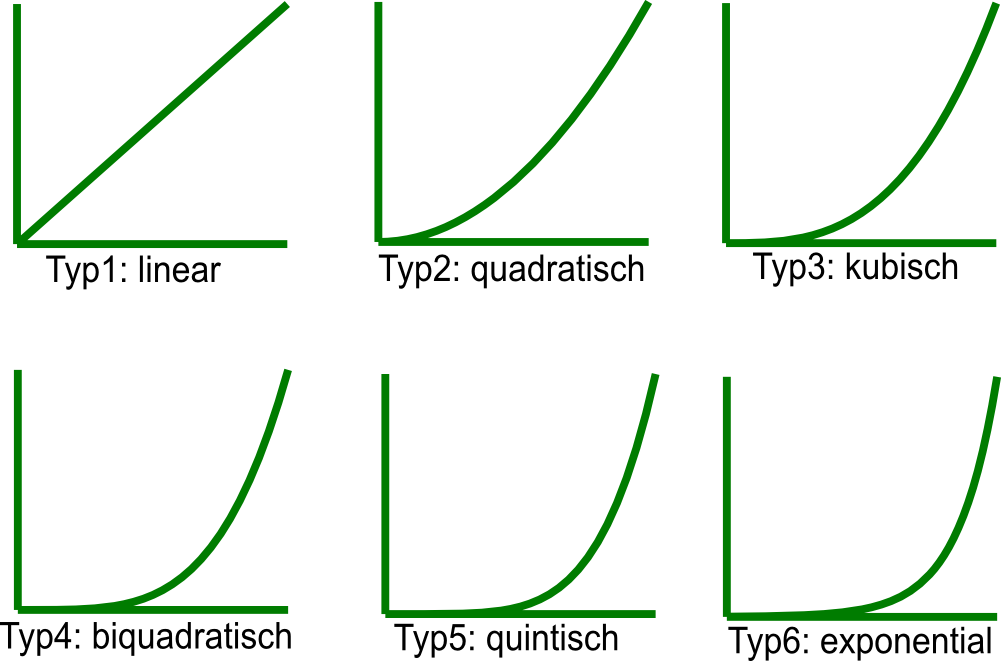
\includegraphics[scale=1.4]{../graphics/curvetypes}
\caption{Die 6 Kurventypen die VSTForx bietet}
\label{curvetypes}
\end{center}
\end{figure}






